\documentclass[12pt,a4paper]{article}
\usepackage{graphicx}
\usepackage{tabularx}
\usepackage{minted}
\usepackage{amsmath}
\usepackage[printonlyused, nohyperlinks]{acronym}
\usepackage{amssymb}
\usepackage{listings}
\usepackage{tikz}
\usetikzlibrary{arrows,positioning, shapes}
\tikzset{
    %Define standard arrow tip
    >=stealth',
    %Define style for boxes
    drect/.style={
           rectangle,
           rounded corners,
           dashed,
           draw=black, thick,
           text width=6.5em,
           minimum height=2em,
           text centered},
   goval/.style={
          circle,
          draw=black, very thick,
          text width=6.5em,
          minimum height=2em,
          text centered},
    % Define arrow style
    pil/.style={
           ->,
           thick,
           shorten <=2pt,
           shorten >=2pt},
    arr/.style={
           ->,
           thick,
           shorten <=2pt,
           shorten >=2pt
           },
    dashedarr/.style={
            ->,
            thick,
            shorten <=2pt,
            shorten >=2pt,
            dashed
    }
}

\usepackage[]{natbib}
\usepackage{float}
\usepackage{glossaries}
\usepackage[hyphens]{url}
% \usepackage[german]{babel}
\usepackage[british]{babel}
\usepackage[utf8]{inputenc} %für Umlaute äüöß
\usepackage{array}
\usepackage[bookmarks]{hyperref}
\graphicspath{{img/}}


%adapting the article class to Ketter requirements
%\usepackage{showframe}
\usepackage[left=5cm, top=2cm, bottom=2cm, right=2cm]{geometry}
\usepackage{setspace}
\onehalfspacing

\lstset{
    basicstyle=\footnotesize,        % the size of the fonts that are used for the code
    breakatwhitespace=false,         % sets if automatic breaks should only happen at whitespace
    breaklines=true,                 % sets automatic line breaking
    captionpos=b,                    % sets the caption-position to bottom
    % deletekeywords={...},            % if you want to delete keywords from the given language
    % escapeinside={\%*}{*)},          % if you want to add LaTeX within your code
    % frame=single,                    % adds a frame around the code
    keepspaces=true,                 % keeps spaces in text, useful for keeping indentation of code (possibly needs columns=flexible)
    %  keywordstyle=\color{blue},       % keyword style
    numbers=left,                    % where to put the line-numbers; possible values are (none, left, right)
    numbersep=5pt,                   % how far the line-numbers are from the code
    rulecolor=\color{black},         % if not set, the frame-color may be changed on line-breaks within not-black text (e.g. comments (green here))
    showspaces=false,                % show spaces everywhere adding particular underscores; it overrides 'showstringspaces'
    showstringspaces=false,          % underline spaces within strings only
    showtabs=false,                  % show tabs within strings adding particular underscores
    stepnumber=1,                    % the step between two line-numbers. If it's 1, each line will be numbered
    tabsize=2,                       % sets default tabsize to 2 spaces
}



%\title{TODO Find best: Social Artificial Neural Network Learning\\
\title{Observation-based Reinforcement Learning Within Competitive Simulations\\
\small{Proposal for Master Thesis}}

\author{Pascal Brokmeier}

\begin{document}
\pagenumbering{arabic}
\maketitle

\section{Motivation}

% TEXT START
\ac{AI} is one of the most discussed technology of the last years. Recent machine learning algorithms allow computers to reliably classify many object classes in images \cite{krizhevsky2012imagenet} through supervised learning but also allow robotics to employ \ac{RL} which let humanoids learn to walk reliably and even perform back-flips \cite{proximalpolicyopt}.

There are many motivations to advance the abilities of machine learning. Examples include: Autonomous vehicle control such as cars or helicopters \cite{abbeel2010autonomous}, autonomous agents helping to balance the complex electricity grids of the future \cite{peters2013reinforcement}, widely available technologies such as image classifications for consumer cloud storage and Consumer recommendation engines for online advertising. \ac{RL} specifically offers the ability to let machines perform complex operations without the need to provide thousands or sometimes millions of labeled examples as is often required for supervised learning methods. They have been shown to quickly learn actions from only very few demonstrations which could allow humans to demonstrate an action that is then mimicked by a \ac{RL} based agent \cite{duan2017one}.

Interestingly, most approaches, independent of the architecture of the agent, approach the task of learning with one agent in mind \cite[p.694ff]{russell2016artificial}. Yet, humans and animals exhibiting higher forms of intelligence as well as many low intelligence species learn in small to large groups or even swarms. Their knowledge is not only a product of individual intelligence but a result of complex network effects of many individuals influencing and interacting with each other \cite[p.200f]{sloman2017knowledge}.

\cite{sloman2017knowledge} and \cite{wegner1995computer} argue that intelligence, as seen in humans, must not only be attributed to individual intelligence but is also caused due to a constant social interaction between many individuals that lead to cultural and technical advancement because of an emergent \emph{community of knowledge}.

%Humans have always distributed labor among many individuals and more importantly, humans distribute learning tasks to individuals. Everyone has a different learning history and specializes in different tasks. We then influence each others' way of thinking by interacting with each other and observing each other. This is true for children just as it is for complex academic communities. AI agent learning research has not approached the topic with similar environments, relying mostly on single agents \cite{russell2016artificial} or sometimes training a multitude of agents but then selecting the best ones and dismissing the rest \cite{jaderberg2017population}, simply to increase the amount of samples which increase the chance of a well trained example to be found.

%Looking at the research of \ac{AI}, the field or \ac{RL} has long defined approaches towards finding a balance between agents that solely try to do as well as they can \emph{in the current iteration} and those that explore the state space to learn new approaches and solutions to reach higher utilities. Commonly, this is accomplished through a degenerating probability of making a \emph{less than optimal} choice when selecting an action, favoring those actions that lead to yet less explored states \cite[]{russel12016artificial}.

Looking at work done by \cite{bansal2017emergent} and \cite{proximalpolicyopt}, agents of different research groups often need to \emph{relearn} the same skills, due to different architectures, hyperparameters or simply because they have different or extended goals. One major claimed benefit of \ac{AI} however, is the ability for all machines to benefit of what one agent has learned. Hence, agents shouldn't need to rediscover how to perform certain tasks but rather receive this skill from other agents that already solved this problem.

Finally, when looking at the complexity of AI algorithms and agent learning, time and performance constraints are always a key factor for the viability of a theoretical algorithm. An algorithm that has exponential complexity in the number of states of the environment is usually only viable for small problems \cite[p.839f.]{russell2016artificial}, not commonly the problems of real world applications. While many algorithms are highly parallelizable \cite{tensorflow2015-whitepaper}, only the most recent incarnations of freely available software tools and libraries are capable of massive distribution of algorithms like \ac{PPO} across many \ac{GPU} nodes \cite{hafner2017agents}. So, as has long been a tradition in computer science, algorithms need to provide a solution in a reasonable time or alternatively need to be easily parallelizable across multiple cores or systems. Distribution of human labor in societies can be viewed as the equivalent to distributed execution of algorithms in computers.

\section{Research question and possible results}

%While it is impossible to guess (and unethical to determine empirically) how the intellect of a human beings would have developed without any human interaction, it is certain that humans learn and research in groups, draw inspiration and ideas from each other and improve on the work of others. It should therefore be investigated if it is also possible for \ac{RL} agents to learn from each other in such a manner.

%such emergent communities of knowledge can also be observed in the \ac{AI} space. The research question can therefore be roughly sketched as such:
%TODO LEAD TOWARDS THE Research Questions

%\emph{Can best-peer derived training data be used to boost learning performance of reinforcement algorithms in a heterogeneous training environment with multiple neural networks?}

%\emph{Can neural networks influence and learn from each other and will this lead to emerging effects exceeding the performance of the individuals?}
\subsection{Delineating the content of the work}


%\subsubsection{What should not be part of the work}

I want to investigate if agents can learn more quickly in groups, reaching a level of performance faster than a single agent learning by himself, not improve the performance of a single agent compared to current \ac{SOTA} agents.

%Effects leading to improved performance can be equivalents to human concepts such as \emph{giving tips}, \emph{explaining} or \emph{imitating successful behavior}.

I also intend to not let the agents directly observe the NN weights of each other to learn from but rather just observe each other as a \emph{black box}. Just as humans cannot look at the inner workings of how someone else thinks, I would first like to just let agents observe each others observations and resulting actions.
An agent is, as in the literature, defined according to the setting in a classical \ac{POMDP} =
$ \{ S, A, P, \Omega, R, \mathcal{O}, \gamma, s_0 \}$
with possible states $s_t \in S$,
observations $x_t \in \Omega$,
actions $a_t \in A$,
following state $s_{t+1} \sim P(s_{t+1} \vert s_t, a_t)$,
rewards $r_t \in R$,
conditional observation probability $x_t \sim \mathcal{O}(s_t)$,
discount factor $\gamma$ and
initial state $s_0$.
Another agent can therefore observe a set of state-action pairs of another agent and use this as a supervised learning input. The agent cannot however see the weights $\theta$ which another agent learned in the process of optimizing its parameterized policy $\pi(\theta)$.
This has the benefit that our agent can also learn from adversarial agents present in the same environment as well as agents of different internal structures. This lets agents learn both faster, assuming other agents already posses the desired skills, and allows for a fast leveling of performance for new market entrants, reducing the market entry barriers for intelligent agents in broker environments such as the electricity market.
However, the loss of possible learning opportunity is intuitive. If an agent could actually observe how another agent \emph{thinks} and if it had the ability to learn from this observation, it might learn much faster to behave in the same way.

%\subsubsection{What should be part of the work}

Once the networks have been trained, it can be interesting to investigate their performance as an ensemble rather than individually \cite{opitz1999popular}. Since ensemble methods average the individual votes, the proposed model might benefit less from ensembles, as most votes are likely to be similar. If this is the case, it would be an indicator for the group of agents being prone to concepts of social influence and herding \cite{2015-45614-00120160201, hirshleifer1994blind}, effects commonly observed in human societies.

An adapted form of boosting on the other hand could strongly affect the performance. Boosting is used in supervised learning to generate multiple hypotheses $h_i$ and after generating each hypothesis, increasing the weight of misclassified examples to increase the attention of the next iteration of hypothesis generation. These multiple hypotheses are then used in a weighted ensemble to collectively decide upon the result \cite[p.749 ff.]{russell2016artificial}. Groups of agents could be trained in different environments, facing different challenges. When looking at the utility function, each term can be evaluated individually to observe performance of parts of the overall goal. If one agent performs better in a certain subtask, it could temporarily be incentivized to focus on this skill by increasing the weight of that term. It will learn to perform better, faster, regarding this subtask as it puts more emphasis on this skill. After a number of iterations, the weight can be reset back to the original loss function and it can \emph{teach} the others how to perform well in this subfield. This is related to the concept of \emph{exploration} in \ac{RL} learning, where agents prefer to explore state transitions that they have not previously explored in-depth yet \cite[p.839f.]{russell2016artificial}. This concept however would give the agents the ability to focus on semantically specific skills rather than just state transitions that haven't been explored much.

Finally, because agents can watch other agents behavior and learn from it, they do not need to relearn the same skills through tedious (and computational expensive) trial and error but rather just imitate the behavior of successful peers, while still retaining the architecture of a generalizing and \ac{RL} based agent. This can both save ramp-up time for new agents and save computational resources with can then be reused for further improvements to the agents through other means.

Based on the previously enumerated motivations and observations, AI research breakthroughs in recent years, similarities between human labor division and multi-threaded execution of algorithms, intelligence emerging from social interactions and connections and the complexity constraints inherent in contemporary learning algorithms, the question arises if agent learning processes can be adapted to more closely resemble the environment in which humans learn. The condensed research question therefore goes as follows:

\emph{Can \ac{RL} agents learn from other agents in the environment? If so, how? Can mutual learning and imitation allow for boosted performance of reinforcement algorithms within a competitive simulation environment?}

\subsection{Conceptual sketch of new learning model}

To let multiple agents learn from each other, the following iterative loop is a sketch of a possible approach:



\begin{enumerate}
    \item Multiple agents are acting in a joint competitive environment. Every agent sees the environment (and the included agents) as a \ac{POMDP}.
    \item After a number of iterations, the agents performances are compared by

\begin{enumerate}
    \item copying
    %we are taking the state at t, the resulting action at t plus the
    $s_{t,i},a_{t,i},r_{t+1,i},x_{t+1,i},p_{t,i}$ from one agent $i$ and
    \item passing them into $\pi_{t,j} \forall j \in N $ of the other agents N at time-step $t$,
    \item  observing if $ U(s_{t+1,j} \vert \pi_{t,j}(s_{t,j}, p_t) \leq U(s_{t+1,i} \vert \pi_{t,i}(s_{t,i},p_t))$ for a benchmarking environment where $P, \mathcal{O}$ are known.
\end{enumerate}
    \item  If another agent is better than the learning agent, the learning agent uses backpropagation and the set of $s_i,a_i$ pairs of the best-peer as supervised learning examples.
    \item repeat
\end{enumerate}

\section{Research approach}


To answer the research question, I propose the following steps:

\paragraph{A literature review} of the involved fields of research is required. Classic and modern learning theories in human psychology and cognitive science as well as current AI research need to be investigated. A special focus will be placed on \ac{RL}.

%\item The concept of emergence needs to be understood. I several networks interacting with each other ought to be investigated, it is important to understand what emergent patterns commonly occur in networks of agents and hence how to facilitate them

\paragraph{The development of a model}
to allow individual agents to observe each other and interact with each other during their learning phases. Current models and software packages do not intend these kinds of interactions among many individual agents, although some work has been done towards this idea \cite{duan2017one}. Hence, it might be necessary to adapt some packages to allow for a more customized loop of learning approaches. A good starting point seem to be the TensorFlow and Gym libraries by Google and OpenAI \cite{tensorflow2015-whitepaper,openaigym}.

\paragraph{Experiment}
 based on the proposed model to determine if the hypotheses hold true.
%For this, common benchmark tasks and datasets can be used to compete with current state of the art architectures.
\citeauthor{openaigym} have created a virtual 3D benchmark environment for \ac{RL} algorithms which can be integrated into python development pipelines. This is a good base to work with, as there has already been work that places multiple agents in a competitive environment \cite{bansal2017emergent}.
%\citeauthor{hafner2017agents} have adapted the virtual 3D gym from OpenAI and made it possible to apply it to highly scaled systems employing the TensorFlow library.
\citeauthor{ketter2016powertac} run a yearly competition for intelligent broker agents acting in a simulated electricity market. This environment is especially interesting, because the agent can be trained with multiple other agents that are publicly available. A socially learning agent can be trained with other agents from previous years and learn to imitate their behavior as long as they perform better than him until it catches up, at which point it may employ the regular forms of learning such as modified policy iteration \cite[p.657]{russell2016artificial} or \ac{PPO} \cite{proximalpolicyopt}.


%\section{Hypotheses to investigate}

\section{Sources and related work}
A preliminary investigation has spawned the following sources as potential input to the development of the thesis.

\subsection{Psychology literature}
Especially in the field of Psychology, the classic views of an individual capable of acting rationally by itself need to be compared to a different direction in Cognitive Psychology: \emph{Transactive Memory Systems}, introduced by \citeauthor{wegner1995computer} and the idea of a \emph{Community of Knowledge} described by \citeauthor{sloman2016cok}. These suggest complex interaction between individuals and their environment.
%What economists often like to think of as \emph{Homo Economicus}, the truly rational agent, these theses suggest there is a much larger dependence on our peers than we might think.
While humans are considered to posses \emph{general intelligence}, the extend to which we as an individual posses this intelligence and not the community as a whole is an interesting field of research
\footnote{I note that I have to broaden my search in this field. The preliminary work has been focused on the AI research, as this is where the core contribution of this work will be. I am aware of cognitive science research about the social aspects of intelligence and knowledge from previous classes however.}.
%\ac{RL} algorithms mostly focus on single agents acting in an environment \cite[p.693ff.]{russell2016artificial}, but recent research puts multiple agents in the same environment, letting them learn in an environment where both agents act in parallel \cite{bansal2017emergent}. This dramatically increases the complexity of the environment from the perspective of the learning agent.

%The agents, while learning separately, will most likely converge in performance, as they copy behavior from each other in regular intervals. This makes the field of social influence as discussed by \citeauthor{hirshleifer1994blind} and information cascades \cite{2015-45614-00120160201} interesting to investigate. While each agent might learn faster, adding many in a group and letting the group decide will likely provide little benefit, as their learning history is so tightly related.

%\subsection{Game Theory}
%TODO basic sources of classic game theory that is often used in virtualized environments for agent learning.

%\subsection{Network Theory / Emergence / ...}
%TODO


\subsection{\ac{AI} Literature and \ac{SOTA} Reinforcement Learning}

\paragraph{\citeauthor{russell2016artificial}}
greatly summarize the state of AI research around 2013. It also gives insights into several fields that influence machine learning and introduces many core architectures for neural networks and \ac{RL}. It can therefore be seen as the core source for the background and theory section of the thesis. Since then, many advances have been made in the field of Neural Networks, triggered by \citeauthor{krizhevsky2012imagenet} paper about image classification with convolutional neural networks.

\paragraph{\citeauthor{bansal2017emergent}}
show the effect of putting several agents in a fairly simple environment, causing large complexity increases in the learning environment through active agents. They interact with each other in the learning environment and often have opposing goals. However, they don't communicate their intention to each other or try to advance each other, meaning that their utility function does not include the value of each other's utility function. Hence they have no reason to help each other, making it a competitive environment. This concept is shown in \autoref{fig:competitiveschema}.

\begin{figure}[H]
    \centering
    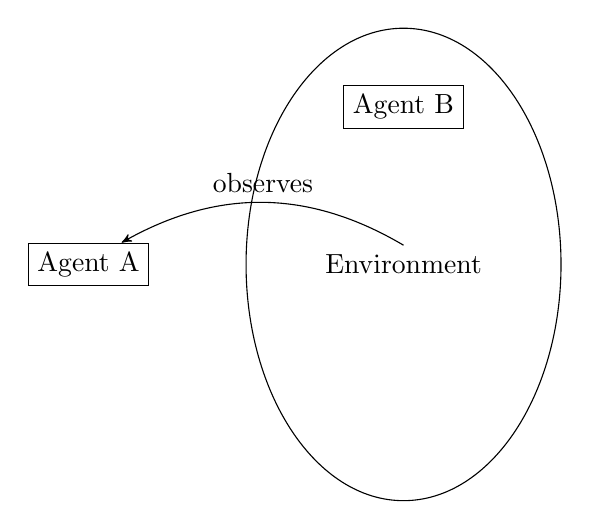
\begin{tikzpicture}[node distance=1cm, auto,]
    % ENVIRONMENT
    \draw (4,0) circle [x radius=2cm, y radius=3cm];

    \node[draw, rectangle] at (4,2) (agentB) {Agent B};
    \node[draw, rectangle] at (0,0) (agentA) {Agent A};
    \node[] at (4,0) (env) {Environment};
    \path[<-,draw, bend left=30]
        (agentA) edge node {observes} (env.north);

    \end{tikzpicture}
    \caption{Agent A indirectly observes B, because he is part of his environment}
    \label{fig:competitiveschema}
\end{figure}



\paragraph{\citeauthor{NG2004Apprentice}}
demonstrated a technique to teach an agent by letting him imitate the behavior of an expert through inverse \ac{RL} \cite{NG2000InvReinf}. This technique can be used to let reinforcement based agents learn from examples, similar to that of supervised learning methods.



\paragraph{\citeauthor{duan2017one}}
show another technique of teaching a neural network by providing demonstrations. For this, they perform demonstrations in virtual space, allowing for full observability in a deterministic environment. They explore different architectures and find \emph{Final state with attention} structures to be most effective for their sample tasks. This can be reasoned is due to the simple final state of the task which does not require multiple complex intermediary steps for which an LSTM network might have gotten better performance.
This work is helpful to understand how an agent can learn from a demonstration in virtual space, adapting itself to achieve the same results. Both this and the work of \citeauthor{NG2004Apprentice} are sketched in \autoref{fig:apprenticeschema}.

\begin{figure}[]
    \centering
    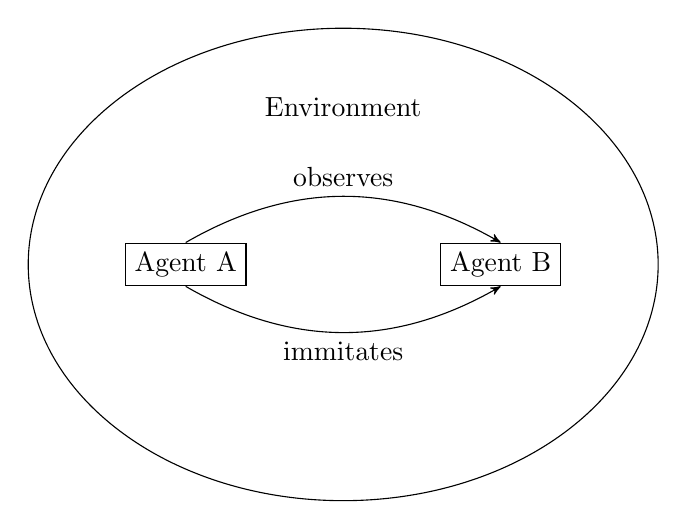
\begin{tikzpicture}[node distance=1cm, auto,]
    % ENVIRONMENT
    \draw (0,0) circle [x radius=4cm, y radius=3cm];

    \node[draw, rectangle] at (2,0) (agentB) {Agent B};
    \node[draw, rectangle] at (-2,0) (agentA) {Agent A};
    \node[] at (0,2) (env) {Environment};
    \path[->, bend left=30]
        (agentA.north) edge node {observes} (agentB.north);
    \path[->, bend right=30]
        (agentA.south) edge node [below]{immitates} (agentB.south);

    \end{tikzpicture}
    \caption{Agent A directly observes B, and learns from him}
    \label{fig:apprenticeschema}
\end{figure}


\paragraph{\citeauthor{jaderberg2017population}}
 show an efficient way of optimizing hyperparameters by letting a population of models exploit each others hyperparameter configurations on-the-fly during learning. For this, a large amount of models are trained in parallel with varying hyperparameters. Those which perform worse copy the values of the hyperparameters of the ones that perform better and continue their training with the new parameters but keeping their previously trained weights. This is visualized in \autoref{fig:populationtraining}.

\begin{figure}[]
    \centering
    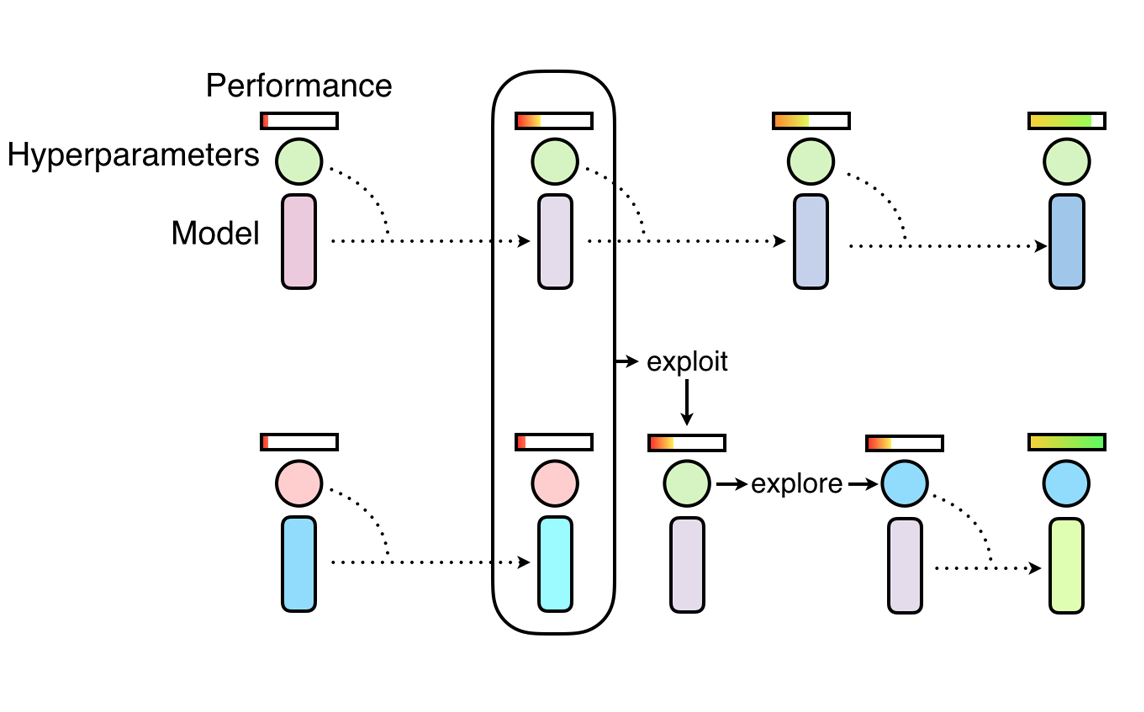
\includegraphics[width=0.7\textwidth]{population_based_hyperparameters.png}
    \caption{Hyperparameter adoption in population based training \cite{jaderberg2017population}}
    \label{fig:populationtraining}
\end{figure}

\paragraph{\citeauthor{foerster2017learning}}
 show how to allow multiple agents learning in a reinforcement environment to achieve the Nash equilibrium for multiple game theory based games. For this they allow each agent to anticipate another agents learning progress and include this anticipation into their own decision for future action. This work is interesting, because it let's agents understand other agents behavior and then act upon it. An example is shown in \autoref{fig:anticipatelearning}, where  two cars heading towards each other evade each other based on the "evade to the right" rule. Agent A can anticipate the action of B and therefore increase its utility. By adapting this model, an agent can understand what another agent does.

From this, the utility function can be easily estimated and if it is reasonably close to its own utility function, the same intentions can be assumed, hence it can serve as a role-model if the performance is superior to the agents own performance.

\begin{figure}[H]
    \centering
    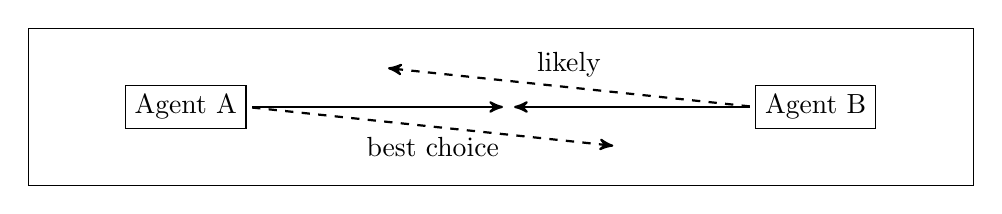
\begin{tikzpicture}[node distance=1cm, auto,]
    % ENVIRONMENT
    \draw (-6,-1) rectangle (6,1);

    \node[draw, rectangle] at (4,0) (agentB) {Agent B};
    \node[draw, rectangle] at (-4,0) (agentA) {Agent A};

    \path[arr] (agentB.west) edge node[below]{} (0.1,0);
    \path[dashedarr] (agentB.west) edge node[above]{likely} (-1.5,0.5);

    \path[arr] (agentA.east) edge node[above]{} (0.1,0);
    \path[dashedarr] (agentA.east) edge node[below]{best choice} (1.5,-0.5);

    \end{tikzpicture}
    \caption{Agent A anticipates move of Agent B and acts accordingly}
    \label{fig:anticipatelearning}
\end{figure}

\paragraph{\citeauthor{ketter2016powertac}} introduced a \emph{"competitive simulation that models a 'liberalized' retail electrical energy market,
where competing business entities or 'brokers' offer energy services to customers through tariff
contracts, and must then serve those customers by trading in a wholesale market."}

This simulation is a great environment to test the ability of \ac{RL} agents in a complex, yet semi-realistic environment which has direct business-applicability. If an agent can perform sufficiently well to compete with other agents and also attain the ability to learn other agents behavior to ensure it doesn't get left behind, this can mean a substantial ability to allow firms to deploy such brokers which generate both revenue and ensure a stable, decentralized electricity grid. A high-level sketch of the game design is shown in \autoref{fig:powertac}.

\begin{figure}[]
    \centering
    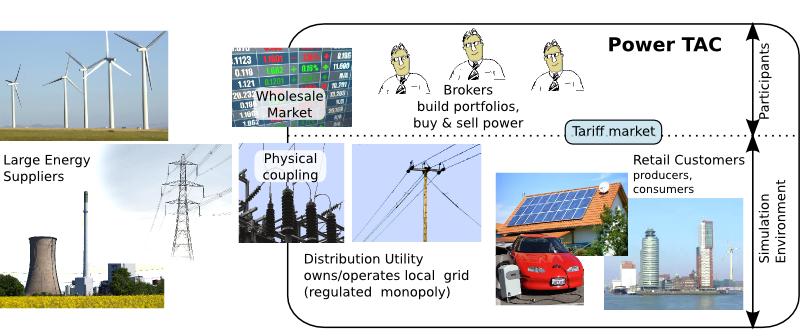
\includegraphics[width=0.85\textwidth]{PowerTAC-scenario.png}
    \caption{PowerTAC game visualization by \cite{ketter2016powertac}}
    \label{fig:powertac}
\end{figure}

\citeauthor{peters2013reinforcement} developed an agent, acting as a broker in this environment. Many other subsequent teams have participated in this simulation and contributed their agents as well. The original agent from \cite{peters2013reinforcement} is based on SARSA, a Q-Learning derivative as well as a linear function approximation approach to compensate for the large state-space which would not be feasible for a simple lookup-table based learning agent. They do note alternative function approximations are available. One such alternative is the neural network approach that has gained a lot of traction in many papers in 2017, such as the following three.

\paragraph{\citeauthor{proximalpolicyopt}} introduced \emph{\acf{PPO}} algorithms, which elaborates on previous work combining neural networks and \ac{RL}. It tries to improve on previous work with policy gradient algorithms which have shown large sample complexity and low data efficiency. To do this, it optimizes a surrogate objective which is more robust against variance in the policy updates by penalizing large deviations of $\frac{\pi_\theta}{\pi_{\theta_{old}}} = 1$ which means penalizing large policy updates, reducing noise while still allowing for sufficient convergence speeds. It also batches updates of several time-steps for its updates, allowing for better data efficiency compared to previous policy gradient algorithms. The final optimization is then a commonly used stochastic gradient descent.


%TODO Expand on emergent complexity
\paragraph{\citeauthor{bansal2017emergent}} extended the work of \cite{proximalpolicyopt} and developed a set of environments for the OpenAI gym library where multiple agents compete against each other in simulated 3D world experiments. The work is interesting, because it shows the arising complexity in simple environments, when multiple non-trivial agents are introduced. This form of self-play allows the training of complex agent behavior without first having to define a complex environment.

They focus on 1-vs-1 games but note that more agents can be added and use a form of exploration factor in the reward functions which initially reward simple motor skills such as standing and walking and slowly transition towards the sparse game rewards which occur much less often. This is because agents initially cannot walk or run and need to learn this first before being able to perform complex tasks like kicking a ball into a goal.

What makes this work also interesting is the problems that researchers face: While previous work regarding teaching such agents the skill of walking, running and jumping exists \cite{heess2017emergence,proximalpolicyopt}, it seems this skill is not easily transferable from one learned agent to another if it is constructed with different techniques or parameter numbers. This causes heterogeneous agents to have the same problem that humans face: Each new individual has to relearn the same skills.

%TODO Tensorflow paper on Gym * 100GPU
\paragraph{\citeauthor{hafner2017agents}} performed some technical work to improve the scalability of the previously introduced \ac{PPO} based reinforcement agents. They adapted the work of \citeauthor{proximalpolicyopt} by vectorizing the agents learning operations and running them in the TensorFlow graph which uses hardware acceleration such as \ac{GPU} or \ac{TPU} chips or clusters. They also allow the parallel execution of multiple OpenAI gym environments. In conclusion, the work allows to overcome the hurdle of the slow learning cycle for environments in which time steps are fixed by instantiating multiple environments in parallel and sending the agents actions to all environments and receiving all observations which are batched and applied as batches in the training algorithm.


\newpage
%Bibliography
\bibliographystyle{apalike}
\bibliography{bibliography}

\end{document}
